% 한국어판 ACL 조판 — tectonic main_ko.tex (XeTeX + kotex). 정본은 영어판 main.tex.
\documentclass[11pt]{article}
\usepackage[review]{acl}
\usepackage{kotex}
\setmainhangulfont{Apple SD Gothic Neo}
\setmonohangulfont{Apple SD Gothic Neo}
\usepackage{graphicx}
\usepackage{booktabs}
\usepackage{amsmath}

\title{암기가 아니라 적용을 배운다: \\ 정책-인-컨텍스트 파인튜닝은 처음 보는 조직 정책에 일반화된다}

\author{Anonymous \\ \texttt{draft v0.6 ko --- not for distribution}}

\begin{document}
\maketitle

\begin{abstract}
조직에서 올바른 행동은 조직의 일정으로 바뀌는 문서가 정의한다; ``조직의 방식대로'' 결정하는 AI는 명문 정책을 따르고, 적용한 규칙을 인용하며, 정책이 재량을 열어둔 곳에서만 위임해야 한다. 지배적인 파인튜닝 레시피는 특정 정책을 모델 가중치에 내재화하는데, 이는 정책이 바뀌는 순간 무너진다. 우리는 반대 프레이밍을 연구한다: 정책은 추론 시점에 \textbf{컨텍스트로} 공급하고, 소형 모델에는 \textbf{주어진 정책이 무엇이든 그것을 적용하는 기술}을 파인튜닝으로 가르친다. 선언적 온톨로지 위의 결정론 규칙 엔진이 생성한 조직 결정 34개 사례(라벨된 판단 3{,}400건) 코퍼스에서, QLoRA로 튜닝한 7B 모델은 훈련에서 본 적 없는 정책에 대해 \textbf{정확 일치 72.9\%}(판정·라우팅·파라미터·\emph{올바른} 인용 규칙)를 달성한다 --- 모든 정책이 정확히 한 번씩 unseen이 되는 leave-case-out 기준이며, 동일 서빙 조건의 미훈련 모델 15.0\%와 대비된다(클러스터 부트스트랩 95\% CI $[64.7, 80.9]$ vs $[3.3, 26.7]$). 무엇을 배웠는지는 통제 3종이 확정한다: approve/reject를 뒤집고 뒤집힘이 답을 바꾸는 레코드만 평가해 \textbf{사전지식이 구조적으로 0점}이 되는 \textbf{반사실 정책}에서 튜닝 모델은 \textbf{88.0\%}를 기록하고, 3-shot 인-컨텍스트 학습 베이스라인은 50.0\%에 그치며, 훈련 시드 분산은 $\pm$4.8pp다. 음성 통제가 레시피의 경계를 긋는다: \emph{같은} 레시피를 바이트 정확 산술 파생 과제에 적용하면 0/6 --- 계산 과정을 타깃에 넣어도, 도구 없는 프런티어 모델을 동일 프롬프트로 평가해도 0/6이며(둘 다 고정밀 나눗셈 필드에서만 실패), 이는 파생이 추론 밖에 속함을 확인한다: 실행마다 도구를 호출하는 것이 아니라 코드로 컴파일해 반복 실행에서 LLM을 아예 제거하는 것이다. 파이프라인이 조직이 이미 지불한 작업 세션으로부터 컴파일되므로, frontier 토큰 손익분기는 \emph{두 번째 실행}이다.
\end{abstract}

\section{서론}

조직에서 무엇이 올바른 일 처리인지는 문서가 정한다. 결정 정책, 지원 런북, 에스컬레이션 매트릭스, 채점 루브릭, 편집 스타일 가이드, 컴플라이언스 체크리스트가 다 그런 문서다. 그리고 이 문서들은 모델이 아니라 조직의 사정에 따라 수시로 바뀐다. 그래서 문서 위에 AI를 세우려면 두 가지를 갈라놓아야 한다. 문서의 \textbf{내용}, 즉 문서가 오늘 말하는 것은 프롬프트 컨텍스트에 둔다. 바뀌는 날 바로 갈아끼우기 위해서다. 반면 그런 문서를 읽고 눈앞의 사안에 충실히 적용하는 \textbf{기술}은 모델 가중치에 넣어 훈련할 수 있다. 이 논문이 측정하는 것이 바로 그 기술이다. 소형 모델이 지도 파인튜닝으로 이 기술을 배우는가, 배웠다면 훈련 때 본 적 없는 문서에도 통하는가.

이 분해는 실무에서 이렇게 굴러간다. 회사의 담당자는 프로그램을 짜거나 모델을 고르는 전문가가 아니다. 처음에는 자기 직군의 일 --- 견적, 환불 승인, 장애 분류 --- 을 에이전트와 대화하며 그냥 해낸다. 그런데 그 대화 기록에는 그 일의 정책과 계산법과 판단 방식이 이미 들어 있다. 이를 선언적 작업 언어(OpenWorkLang)로 표현하고 컴파일러(OpenWorkCompiler)를 돌리면 정책은 온톨로지와 규칙이 되고, 계산은 프로그램이 되고, 판단은 훈련된 소형 모델이 맡는다. frontier LLM 없이 로컬 GPU만으로 특수 목적 업무에 충분한, 토큰이 크게 절약되는 업무 수행·결정 도구가 만들어지는 것이다. 이 논문은 그 사슬에서 가장 의심스러운 고리 하나를 실험으로 확인한다. 판단이 정말 소형 모델에 학습되는가 --- 나머지 고리(계산은 프로그램으로, \S\ref{sec:control}; 토큰 경제, \S\ref{sec:economics})는 통제와 실측으로 뒷받침한다.

이 부류에서 결정론 채점이 되는 가장 깨끗한 사례가 조직의 결정 정책이라, 우리는 그것을 연구한다. 직원이 ``이 고객에게 12\% 할인을 줘도 되나요?''라고 물을 때 조직이 원하는 답은 어느 똑똑한 모델의 의견이 아니다. \emph{조직 자신의 정책이 적용된 결과}다. 순서 있는 규칙을 위에서부터 검사하고, 처음 걸리는 규칙을 인용하고, 정책이 지정한 승인자에게 넘기고, 정책이 일부러 열어둔 재량 밴드(``5--10\%: AI 추천 가능, 팀장 승인'')만 추천으로 채우는 것. 여기서 ML 문제의 조건 세 가지가 나오는데, 셋 다 위의 분해를 그대로 보여준다:

\begin{enumerate}
  \item \textbf{문서는 모델보다 빨리 바뀐다.} 정책 $P$를 암기한 모델은 $P$가 $P'$이 되는 날 틀린다. 그러니 내용은 가중치 바깥에 두어야 한다.
  \item \textbf{판단은 감사 가능해야 한다.} ``승인''만으로는 답이 아니다. ``승인, 본부장 라우팅, \texttt{strategic\_retention\_band} 인용, 그 조건이 이 레코드에 실제로 성립''까지가 답이다.
  \item \textbf{재량은 선언되는 것이지 추론되는 것이 아니다.} 모델이 어디까지 추천해도 되는지는 문서가 정한다. 신뢰도 임계값이 정하는 게 아니다.
\end{enumerate}

선행 연구는 셋 중 하나를 한다. 정책을 가중치에 내재화하거나 \citep{trimpi2025}, 정책 지침을 준 에이전트를 벤치마킹하거나 \citep{taubench2024,rulearena2024}, 규칙이 개정될 때 얼마나 버티는지 측정한다 \citep{guidebench2025}. 정작 배포 현장이 요구하는 조합은 빠져 있다. \textbf{로컬에서 돌릴 수 있는 소형 모델에 ``어떤 정책이 오든 컨텍스트에서 읽고 적용하는 기술''을 파인튜닝으로 가르치고, 훈련 때 본 적 없는 정책에서 그 기술을 재는 것} 말이다.

선언적 결정 정책을 고른 이유는 둘이다. 적용 기술(순서대로 검사, 첫 일치 적용, 근거 인용)이 만만치 않으면서도, 정답은 바이트 단위로 채점할 수 있기 때문이다. 런북이나 루브릭처럼 더 지저분한 문서로도 이 레시피가 통하는지는 아직 열린 질문이고, \S\ref{sec:discussion}에서 로드맵과 함께 범위를 긋는다.

기여:
\begin{itemize}
  \item \textbf{과제와 코퍼스} (\S\ref{sec:task}): 10개 조직 기능의 결정 사례 34개 --- 온톨로지 + 명시적 재량 밴드를 가진 순서 규칙으로 선언, 결정론 엔진이 인용 규칙·성립 조건이 달린 라벨된 판단 3{,}400건으로 컴파일.
  \item \textbf{엄격한 결정론 채점기} (\S\ref{sec:grading}): 판정·라우팅·파라미터·인용 규칙의 정확 일치 + 인용 규칙의 조건이 레코드에 실제로 성립하는지 검증.
  \item \textbf{전이 결과} (\S\ref{sec:transfer}): 34개 정책 전부의 leave-case-out, 72.9\% $[64.7, 80.9]$ vs raw 15.0\%(동일 bf16 greedy 서빙); ICL 사다리 $15.0 \rightarrow 50.0 \rightarrow 72.9$.
  \item \textbf{반사실 통제} (\S\ref{sec:counterfactual}): 사전지식이 구조적으로 0점인 뒤집힌 정책에서 88.0\%.
  \item \textbf{음성 통제와 배치 경제학} (\S\ref{sec:control}--\ref{sec:economics}): 같은 레시피가 바이트 정확 산술에서 실패(0/6), CoT 타깃 절제에도 유지, 도구 없는 프런티어도 같은 게이트에 실패 --- 실행마다의 tool call을 넘어 코드로 컴파일하는 한 걸음(실측 2회차 손익분기)을 정당화.
\end{itemize}

\section{관련 연구}

\paragraph{정책 내재화 vs 정책-인-컨텍스트.} Multimodal Policy Internalization \citep{trimpi2025}은 정책을 모델 파라미터 \emph{안으로} 훈련해 추론 시 정책이 컨텍스트에 없어도 되게 한다 --- 우리와 반대의 유지보수 베팅이다. 그쪽의 ``Policy Override'' 설정은 갱신된 정책을 추론 시 컨텍스트로 주되 내재화 모델의 \emph{일반화 프로브}로 쓴다; 우리는 컨텍스트 적용 자체를 훈련 목표로 만든다. Policy Reasoning Traces \citep{prt2025}는 HIPAA·GDPR 등 특정 정책의 컴플라이언스 평가를 정책별 인스턴스 분할로 개선하며, 교차-정책 전이는 부수 분석으로만 등장한다 --- 우리의 홀드아웃-정책 프로토콜과 다르다. GuideBench \citep{guidebench2025}는 규칙 개정 강건성을 벤치마킹한다.

\paragraph{정책 준수 벤치마크.} $\tau$-bench \citep{taubench2024}는 도메인 정책 지침을 준 SOTA 에이전트를 평가하고, RuleArena \citep{rulearena2024}의 발견은 규칙 식별 실패와 규칙이 요구하는 계산의 실패를 구분해 우리 \S\ref{sec:control}를 직접 예고하며, CRMArena-Pro \citep{crmarena2025}는 엔터프라이즈 시나리오에서 에이전트를 평가한다. 동시대의 엔터프라이즈 벤치마크 \citep{enterprisebench2026}는 규칙 엔진이 채점하는 결정을 독립 구축했으나 평가 전용이고 재량 밴드가 없다. DMN \citep{dmn2024}은 FIRST-hit 의미론의 순서 결정 규칙을 표준화해 왔다 --- 우리 DSL은 의도적으로 그 계열이며, ML 기여는 규칙 언어가 아니라 전이 측정이다.

\paragraph{SFT와 산술.} Faith and Fate \citep{faithfate2023}는 Transformer가 합성적 다단계 산술에 실패함을 보였고, \citet{sftmemorizes2025}는 SFT가 암기하며 분포 밖에서 고전함을, PAL \citep{pal2022}은 풀이 단계를 파이썬 인터프리터로 넘기는 계열의 원조를 이룬다. 우리의 기여는 부정 결과가 아니라 그 \emph{짝지음}이다: 산술에서 실패한 그 레시피·코퍼스 규모·게이트가 규칙 적용에서는 성공하고, 도구 없는 프런티어가 같은 산술 게이트에 실패해 ``소형 모델은 계산을 못 한다''를 ``추론은 계산을 못 한다''로 벼린다.

\paragraph{소형 모델 배포.} \citet{slmposition2025}은 소형 모델이 에이전틱 AI의 미래라 주장하고 LLM→SLM 전환 알고리즘을 제시한다; 우리는 고가치 슬롯 하나(정책 적용)의 훈련된 기술 레시피와 전이 측정, 그리고 다른 슬롯(파생)에 대해 프런티어조차 실패하는 결정론 게이트를 제공해 선호가 아닌 \textbf{배치 규칙}을 내놓는다.

\section{과제와 코퍼스}\label{sec:task}

\subsection{결정 사례}
\emph{사례}는 반복되는 조직 결정 하나를 선언한다: 결정 역할, \textbf{온톨로지}(개체·속성·관계), 피처 공간, \textbf{순서 규칙}(\texttt{when} 조건 $\rightarrow$ 판정·라우팅·파라미터·사유), 선택적 \textbf{재량 밴드}(\texttt{defer: slm\_recommend}, 밴드 한계는 파라미터로), fallback. 코퍼스는 \textbf{10개 기능(영업·재무·고객지원·인사·구매·법무·IT운영·마케팅·물류·보안)의 34개 사례}를 담는다. 결정론 엔진이 각 사례의 피처 공간에서 레코드를 샘플링하고 첫 일치 의미론을 적용해 \textbf{사례당 라벨된 판단 100건}(총 3{,}400건)을 만들며, 각 판단에 적용 규칙명·조건·사유가 붙는다. 생성은 시드 고정·바이트 재현이다.

\subsection{정책-인-컨텍스트 형식}
모델은 인스턴스마다 조직·역할·결정을 명명하는 시스템 턴, 사례의 온톨로지와 \emph{전체 순서 규칙 목록}(YAML 원문), 레코드를 받는다. 출력은 JSON 객체 하나 --- \texttt{\{verdict, route, params, cited\_rule, rationale\}}. 특정 정책에 관한 무엇도 가중치에 없으므로 규칙 수정은 재훈련 없이 행동을 바꾼다.

\subsection{채점}\label{sec:grading}
답이 \textbf{정확}(exact) 판정을 받으려면 판정·라우팅·파라미터가 엔진의 결정과 같고, \emph{그리고} 인용 규칙이 첫 일치 규칙이며, \emph{그리고} 그 규칙의 조건이 레코드에 실제로 성립해야 한다(마지막 검사는 판정을 찍어 맞혀도 근거 날조를 실패시킨다). \textbf{완화}(relaxed) 지표는 첫 일치가 아니어도 조건이 진짜 성립하는 규칙 인용을 나머지가 전부 정답일 때 인정한다. 판정-단독 정확도도 병기한다. 홀드아웃 항목이 정책 단위로 군집하므로 모든 신뢰구간은 \textbf{사례-클러스터 부트스트랩}(10{,}000회)이다.

\subsection{정직한 범위}\label{sec:scope}
코퍼스는 합성이고 자기 채점이다: 라벨을 만드는 엔진이 채점하는 엔진이고, 정책은 이미 기계가독이며, 규칙 조건의 필드명이 레코드 키와 일치한다 --- 산문 정책의 엔티티 정합 난이도, 결측·노이즈 필드, 주석자 불일치가 부재한다. 따라서 주장은 \emph{선언적 정책 위에서의 정책 적용} 전이이며, 의도적으로 깨끗한 기판이다; 산문 정책으로 가는 길은 \S\ref{sec:discussion}에서 논의한다.

\section{실험 설정}

\paragraph{모델·훈련.} Qwen2.5-7B-Instruct, QLoRA($r{=}16$, $\alpha{=}32$, dropout 0.05, 전체 선형 프로젝션), completion-only 손실, 2 에폭, LR $10^{-4}$ cosine, RTX 4090 1장 bf16($\approx$12분/런). 훈련 데이터: 28사례 $\times$ 40인스턴스(1{,}120행); 6사례는 \emph{통째로} 홀드아웃. 환경은 핀 고정이고 모든 런이 매니페스트(시드·에폭·데이터/어댑터 SHA-256·패키지 버전)를 기록한다.

\paragraph{서빙·공정성.} 튜닝 모델과 raw 베이스라인 \emph{모두} 같은 bf16 서버·greedy 디코딩으로 평가한다. (동일 조건 재평가에서 raw 7B는 16.7\%→15.0\% --- 양자화 교란은 격차를 설명하지 못한다.)

\paragraph{분할.} (a) \emph{고정}: 홀드아웃 6사례 $\times$ 10인스턴스 + seen-정책/unseen-인스턴스 56건. (b) \emph{Leave-case-out(LOCO)}: 같은 레시피로 6-fold 재훈련해 34개 정책 전부가 정확히 한 번씩 unseen(340건, 클러스터 34개).

\section{결과}

\subsection{처음 보는 정책으로의 전이}\label{sec:transfer}

\begin{figure*}[t]
  \centering
  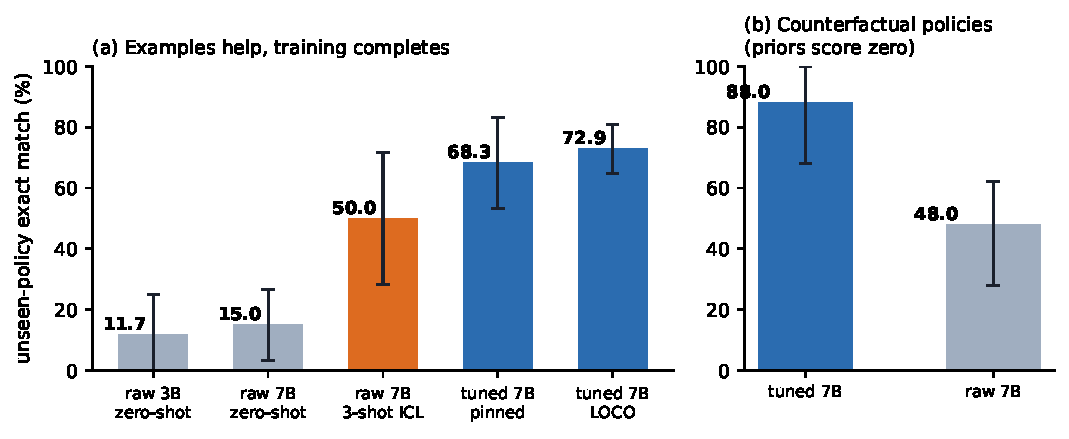
\includegraphics[width=0.98\textwidth]{../figs/fig1_ladder_counterfactual.pdf}
  \caption{(a) 클러스터 부트스트랩 95\% CI가 달린 unseen-정책 정확 일치. (b) 반사실 통제: 뒤집힌 정책이 다르게 결정하는 레코드에서 사전지식은 구조적으로 0점.}
  \label{fig:ladder}
\end{figure*}

\begin{table}[t]\small
  \centering
  \begin{tabular}{@{}lrr@{}}
    \toprule
    모델 (동일 서빙) & 정확 & 95\% CI \\
    \midrule
    raw 3B, 제로샷        & 11.7\% & $[0.0, 25.0]$ \\
    raw 7B, 제로샷        & 15.0\% & $[3.3, 26.7]$ \\
    raw 7B, 3-shot ICL    & 50.0\% & $[28.3, 71.7]$ \\
    tuned 7B (고정 분할)  & 68.3\% & $[53.3, 83.3]$ \\
    \textbf{tuned 7B (LOCO)} & \textbf{72.9\%} & $\mathbf{[64.7, 80.9]}$ \\
    \bottomrule
  \end{tabular}
  \caption{unseen-정책 정확 일치. LOCO는 34개 정책 전부를 정확히 한 번씩 홀드아웃한다.}
  \label{tab:main}
\end{table}

LOCO fold 정확도는 65.0--80.0\%: 고정 분할 결과는 한 분할의 산물이 아니다(표~\ref{tab:main}, 그림~\ref{fig:ladder}a). 훈련 시드 3개에 걸쳐 unseen 정확은 $62.8\% \pm 4.8$pp --- 실행 간 분산은 실재하고 보고되며, 어떤 시드도 raw 베이스라인 근처로 내려가지 않는다. 인-컨텍스트 예시는 크게 돕지만($15 \rightarrow 50\%$) 파인튜닝이 그 위에 ${\sim}20$pp를 더하고 요청마다의 예시 토큰도 없앤다. LOCO의 정책별 성적은 1/10--10/10(그림~\ref{fig:perpolicy}); 조건에 날짜·한도 산술이 든 승인 정책(휴가·초과근무·지급기한 연장)이 최하위에 앉아 \S\ref{sec:control}를 예고한다.

\begin{figure}[t]
  \centering
  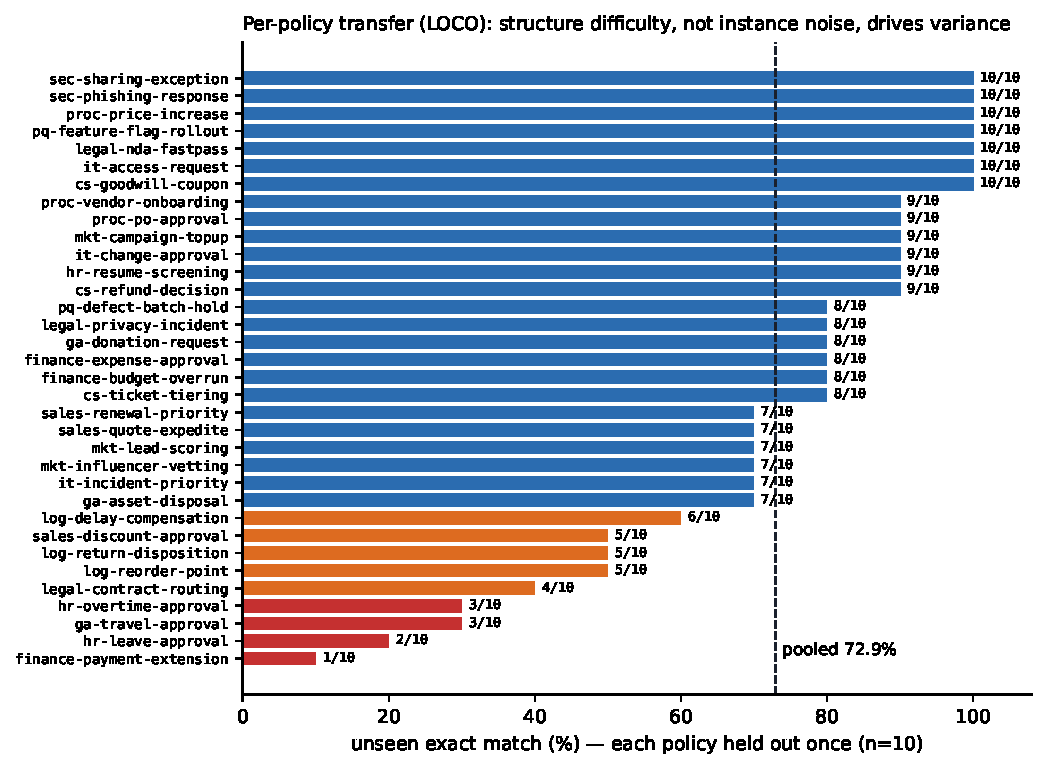
\includegraphics[width=\columnwidth]{../figs/fig2_per_policy.pdf}
  \caption{LOCO 하의 정책별 전이; 모든 정책이 정확히 한 번 unseen($n{=}10$).}
  \label{fig:perpolicy}
\end{figure}

\subsection{무엇을 배웠나: 반사실 통제}\label{sec:counterfactual}
홀드아웃 사례의 모든 규칙(및 fallback)에서 approve$\leftrightarrow$reject를 뒤집고, \textbf{뒤집힌 정책이 원 정책과 다르게 결정하는 레코드만} 평가한다 --- 이 부분집합에서 사전지식이나 원 정책으로 답하면 구조적으로 0점이다. 튜닝 모델은 \textbf{88.0\%}(44/50), raw 7B는 48.0\%(그림~\ref{fig:ladder}b). \S\ref{sec:transfer}와 결합하면, 파인튜닝이 가르친 것은 정책 내용도 세상의 사전지식도 아닌 \emph{컨텍스트 정책의 적용}이라는 직접 증거다.

\subsection{음성 통제: 같은 레시피는 계산을 못 배운다}\label{sec:control}
동일 레시피(같은 트레이너·게이트·코퍼스 규모 300예시)를 같은 제품군의 \emph{파생} 과제 --- 고객 갱신 가격 파일(22개 수치 필드)의 바이트 정확 재생성, 결정론 게이트 채점 --- 에 적용했다.

\begin{table}[t]\small
  \centering
  \begin{tabular}{@{}lrr@{}}
    \toprule
    팔 & 게이트 & 필드 정확도 \\
    \midrule
    SFT 7B (일반 타깃)      & 0/6 & --- \\
    SFT 7B (CoT 타깃)       & 0/6 & 86.4\% \\
    프런티어, 도구 없음     & 0/6 & 93.6\% \\
    \bottomrule
  \end{tabular}
  \caption{산술 음성 통제. 튜닝·프런티어 팔 모두 거의 오로지 나눗셈 2필드에서 실패한다.}
  \label{tab:control}
\end{table}

이것은 \emph{발견이 아니라 통제}다 --- 산술을 도구로 보내는 것은 정착된 관행이다. 역할: (i) ``더 훈련하면 된다'' 반론을 닫는다(CoT 절제에도 실패; 프런티어가 같은 두 나눗셈 필드에서 같은 게이트에 실패하면서 밴드·할인 규칙은 전부 정답; 원 기록 에이전트가 통과한 이유는 도구로 계산했기 때문). (ii) 필드 단위 점수는 exact 게이트가 숨기는 것을 보여준다 --- 추론은 22개 중 20--21개 필드를 맞히며, 실패는 계산이 필요한 곳에만 몰린다. (iii) 표준 처방보다 한 걸음 더: 실행마다의 \textbf{tool call은 매 실행 LLM을 루프에 남긴다}(어떤 도구를 부를지 재결정 --- 토큰·비결정성·재조율), \textbf{code 계층 컴파일은 그 결정을 한 번만} 내린다. 배치 규칙: 파생 $\rightarrow$ code; 정책 판단 $\rightarrow$ 결정론 게이트 뒤의 훈련된 SLM; 선언된 재량 밴드 $\rightarrow$ 추천 + 사람 승인자.

\subsection{배치 경제학: 손익분기는 두 번째 실행}\label{sec:economics}
갱신 파이프라인을 유니크 토큰(턴마다 재전송되는 누적 컨텍스트를 중복 계상하지 않는 기준)으로 실측: 기록된 에이전트 세션은 실행당 frontier 토큰 23{,}614개; 컴파일과 SLM 승격 후 실행은 \textbf{frontier 토큰 0개}(로컬 4{,}208 토큰, 한계비용 \$0, 7.4$\times$ 빠름, 결정론 벤치마크로 7/7 재현). 컴파일러의 입력이 조직이 어차피 한 번은 실행해야 했던 작업 세션이므로 frontier 토큰 \textbf{손익분기는 두 번째 실행}이다 --- 컴파일러가 LLM 토큰으로 탐색하는 최적화 중심 컴파일의 ${\approx}$17-트랜잭션 손익분기 \citep{compiledai2026}와 대비된다. 새 파라미터 값의 에스컬레이션은 각 1회의 frontier 호출 후 상류 출력 지문과 함께 캐시되어 반복에서 0으로 상각된다. 숨은 분모는 온톨로지·정책을 선언하는 사람의 비용이다; 파이프라인은 결정의 반복 빈도에 비례해 성립하며 --- 조직이 가장 먼저 자동화하는 영역 --- record-first 설계가 그 분모를 작게 유지한다.

\section{논의}\label{sec:discussion}

\paragraph{왜 내재화하지 않는가?} 가중치에 내재화된 정책은 빠르게 답하지만 즉시 낡고 규칙 수정을 설명하지 못한다. 정책-인-컨텍스트는 유지보수 경제학을 뒤집는다: 정책 파일이 배포 산물이고, 재훈련은 정책이 아니라 \emph{기술}이 표류할 때만 필요하다.

\paragraph{정책 결정 너머.} 레시피의 무엇도 승인 워크플로 특화가 아니다: 훈련 행은 (문서, 레코드, 근거 있는 구조화 답변) 삼중항이고, 반사실 통제는 의미를 프로그램적으로 뒤집을 수 있는 모든 문서 클래스로 일반화된다. 런북과 루브릭이 최근접 이웃이며, 각자 결정론 채점기가 필요하다 --- 그것이 주장을 넓히는 실제 병목이다(표~\ref{tab:roadmap}). 이 논문은 또한 더 큰 컴파일 파이프라인 시스템의 한 계층이며, 그 종단 경제학(\S\ref{sec:economics})은 전이 결과에 동기를 주지만 의존하지 않는다.

\begin{table}[t]\footnotesize
  \centering
  \begin{tabular}{@{}p{2.3cm}p{2.2cm}p{2.2cm}@{}}
    \toprule
    문서 클래스 & 필요한 채점기 & 현황 \\
    \midrule
    결정 정책 & 규칙 엔진 & \textbf{측정 완료(본 논문)} \\
    에스컬레이션 매트릭스 & 표 조회 & 근접(카탈로그 사례) \\
    컴플라이언스 체크리스트 & 항목별 규칙 & 미착수 \\
    채점 루브릭 & 정답지 & 미착수 \\
    지원 런북 & 상태머신 & 미착수 \\
    \bottomrule
  \end{tabular}
  \caption{content-in-context, skill-in-weights 레시피의 일반화 로드맵.}
  \label{tab:roadmap}
\end{table}

\paragraph{산문 정책으로 가는 길.} 우리 기판은 엔티티 정합을 제거한다(규칙 필드명 = 레코드 키). 자연스러운 다음 실험은 훈련된 applier를 고정한 채 앞에 정책 컴파일 단계(산문 $\rightarrow$ 선언 규칙)를 끼우고, 72.9\% 중 얼마가 노이즈 있는 컴파일을 견디는지, 반사실 통제가 여전히 성립하는지 측정하는 것이다.

\section*{한계}
라벨과 채점이 같은 엔진에서 나온다; 근거-성립 검사, 완화 지표, 반사실 통제, 전체 핀 고정으로 완화했지만 주석자 간 일치도가 있는 사람 라벨 판단은 향후 과제다. 규모: 정책 34개, 베이스 모델 7B 하나, 언어쌍 하나(한국어 프롬프트, 혼합 언어 필드); 클러스터 CI가 이에 정직하다 --- 주장은 72.9\%가 아니라 $[64.7, 80.9]$다. 정책은 이미 기계가독이며 산문 정책의 엔티티 정합은 미검증이다. 프런티어 통제는 프런티어 모델 하나·프롬프트 형식 하나·설계상 도구 없음이다.

\section*{재현성}
코퍼스 생성기, 트레이너(핀 고정·런별 매니페스트), 평가 코드, 모든 원자료와 이 초고가 한 저장소에 있다; 모든 표는 시드 고정 생성기와 저장된 모델 출력에서 재생 가능하다.

\bibliography{refs}

\end{document}
